\subsection{Effect of sparsity on downstream task performance}
\label{app:downstream}

In~\Cref{sec:scaling_law_ds}, we analyzed the relationship between upstream pre-training loss and downstream task performance across different \moe sparsity levels. We found that language understanding and world knowledge tasks generally showed a strong correlation between upstream and downstream performance, while reading comprehension tasks seemed to favor denser models to some extent. 

In this section, we provide additional plots for a broader range of tasks within each category to further support our findings. We consider the following tasks:
\begin{itemize}[left=0pt,itemsep=2pt]
\item \textbf{Common Sense Reasoning}: PIQA, CommonSenseQA, OpenBookQA, COPA
\item \textbf{Language Understanding}: LAMBADA, HellaSwag, Winograd, Winogrande
\item \textbf{Reading Comprehension}: SQuAD, CoQA, BoolQ
\item \textbf{World Knowledge}: TruthfulQA, ARC-Easy, ARC-Challenge
\end{itemize}
\Cref{fig:additional_ds_plots} shows the relationship between upstream pre-training loss and downstream task performance for these additional tasks. Each row corresponds to a task category and each subplot represents a different task, with points colored according to \moe sparsity $S$. The $x$-axis represents the upstream pre-training loss, while the $y$-axis shows the downstream task performance metric (usually accuracy or error rate). These results supplement our main findings from \Cref{sec:scaling_law_ds}:
\begin{itemize}[left=0pt,itemsep=2pt]
    \item We observe consistent trends across tasks within each category, with language understanding and world knowledge tasks showing strong correlations between upstream and downstream performance regardless of sparsity. 
    \item Reading comprehension tasks continue to show a slight advantage for denser models, while common sense reasoning tasks (which can be considered part of the symbolic problem-solving category) show more varied relationships between upstream and downstream performance.
\end{itemize}

\begin{figure}[tbp]
    \centering
    \subfigure{
        \centering
        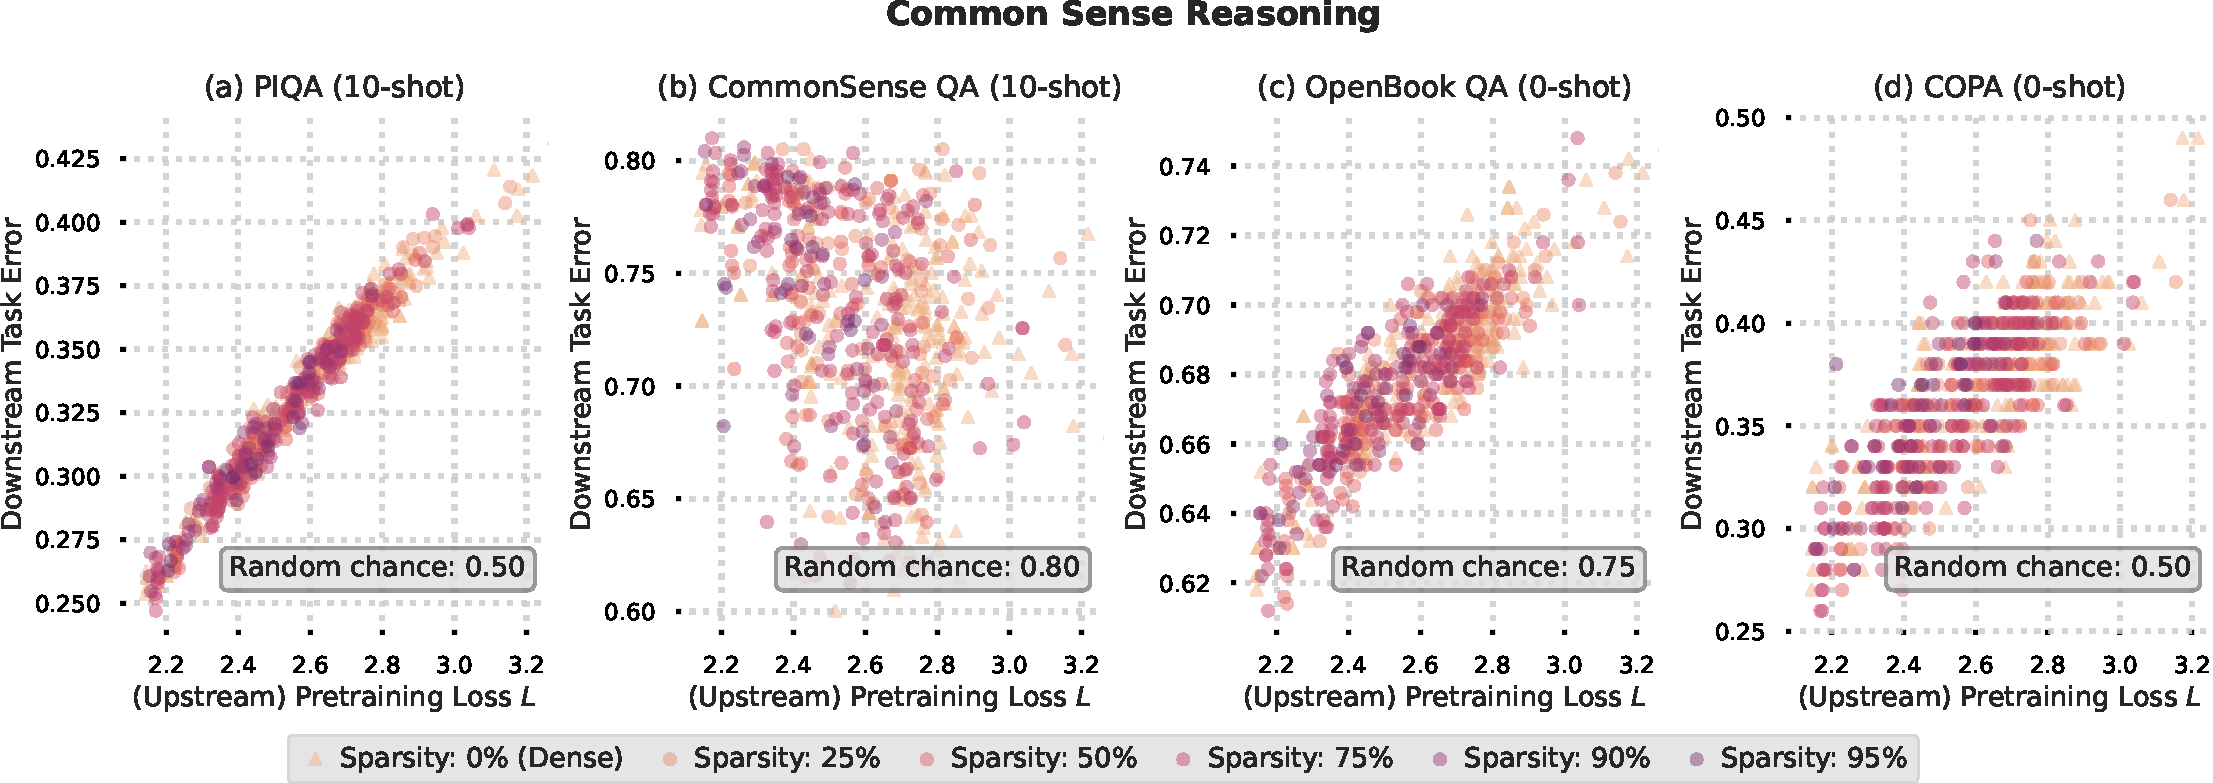
\includegraphics[width=0.75\textwidth]{plots/appendix/app_s4_common.pdf}
        \label{fig:s4_sub1}
}    \subfigure{
        \centering
        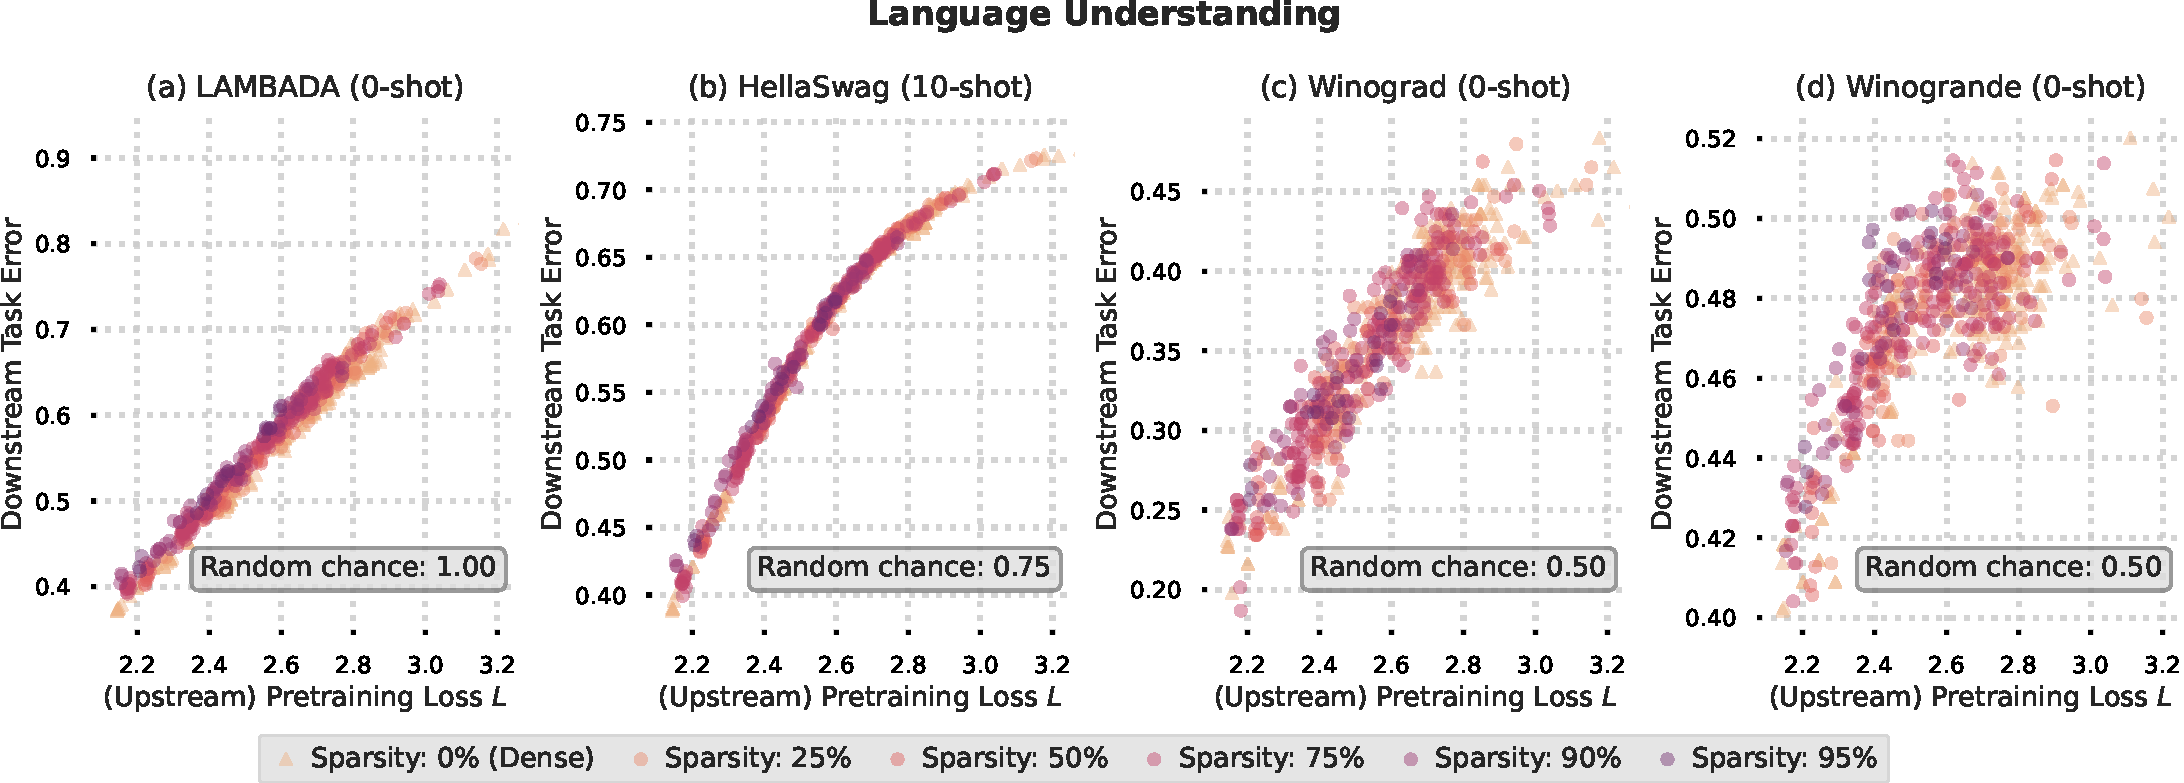
\includegraphics[width=0.75\textwidth]{plots/appendix/app_s4_language.pdf}
        \label{fig:s4_sub2}
}    \subfigure{
        \centering
        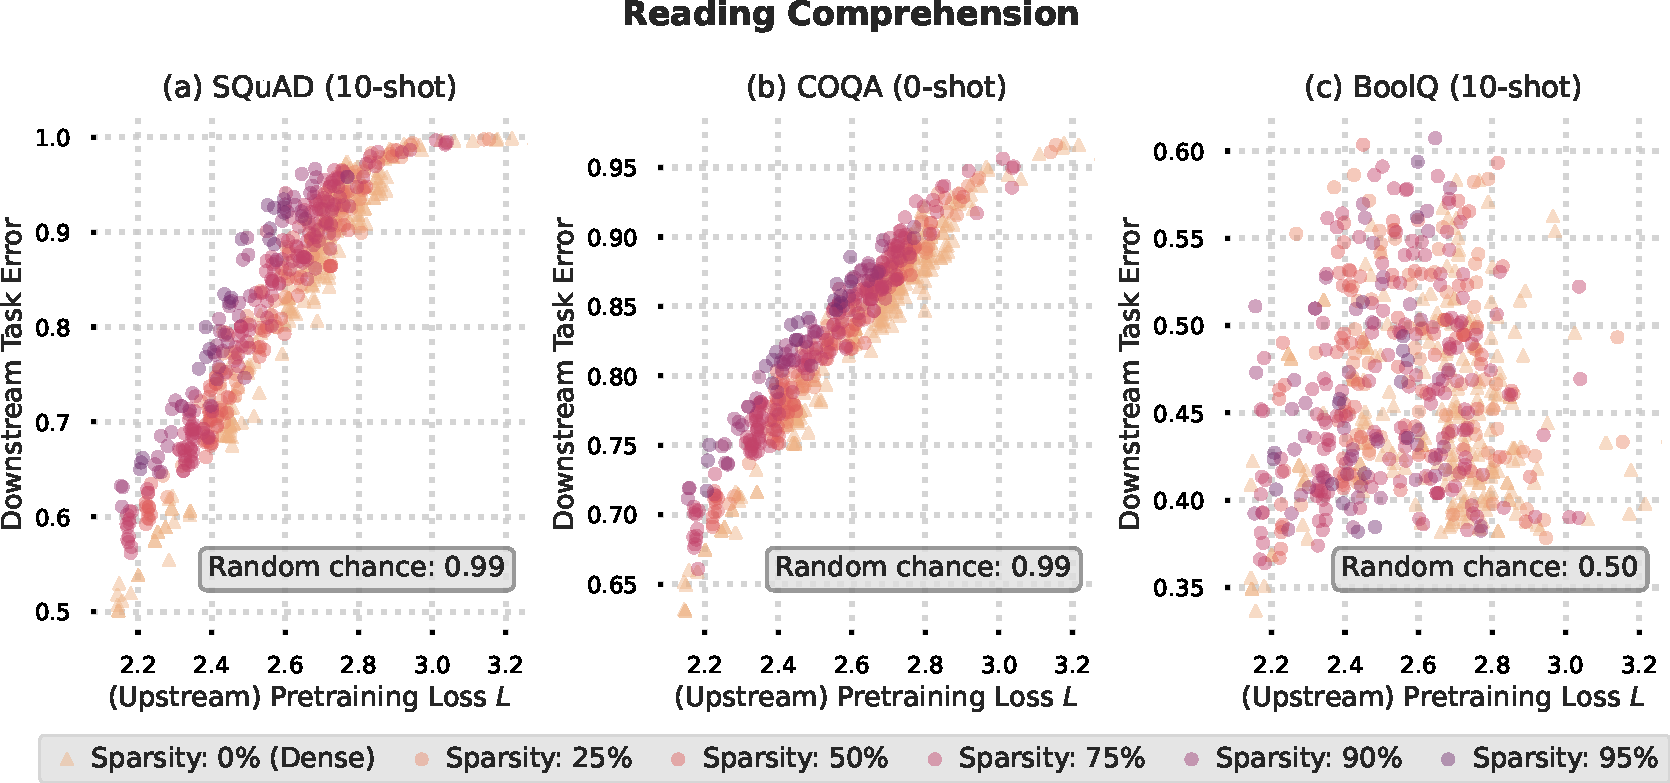
\includegraphics[width=0.6\textwidth]{plots/appendix/app_s4_reading.pdf}
        \label{fig:s4_sub3}
        \par\medskip
}    \subfigure{
        \centering
        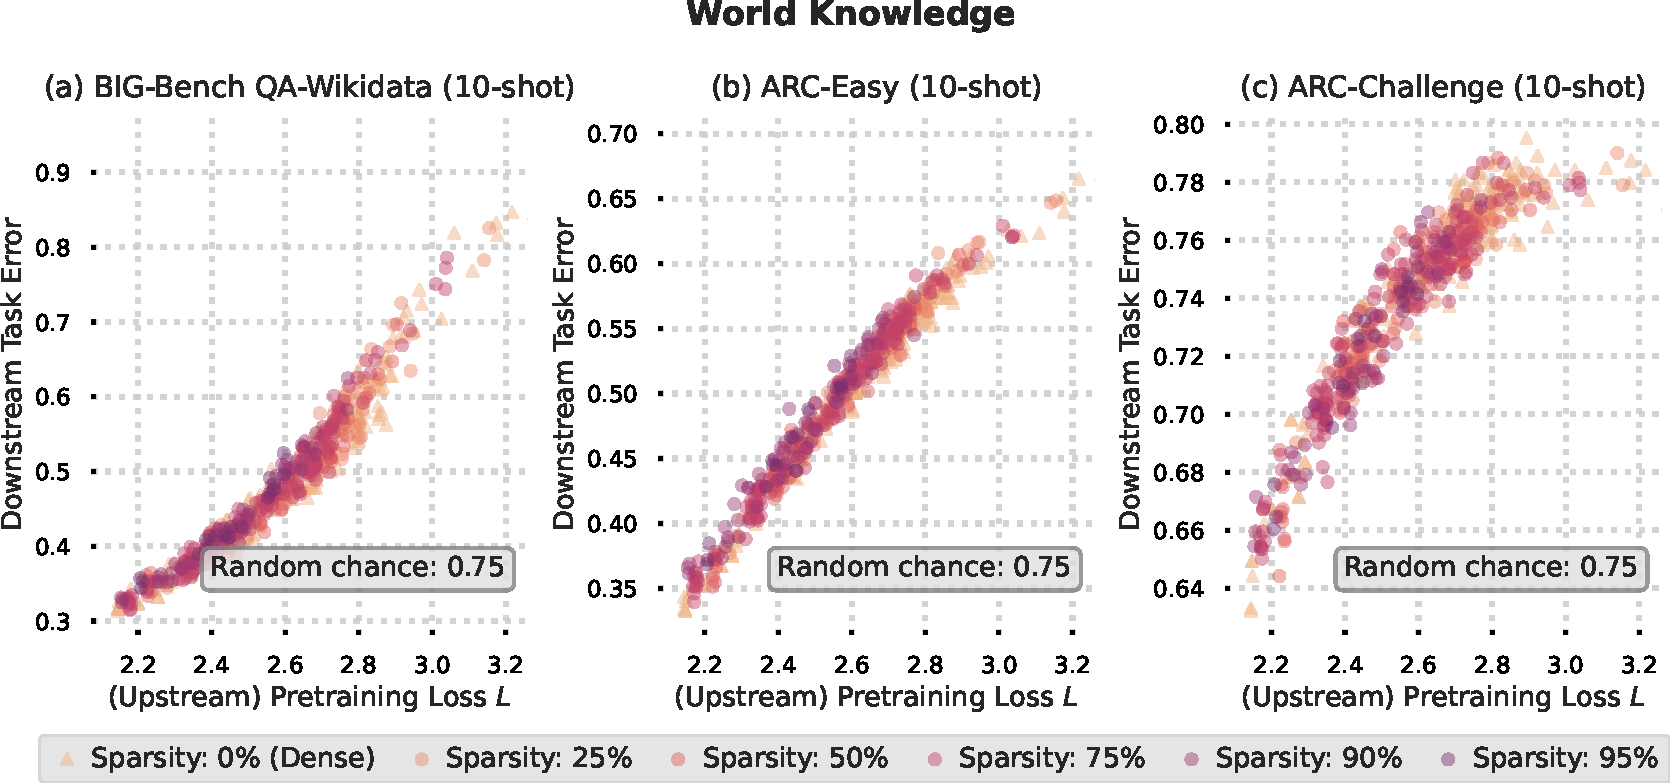
\includegraphics[width=0.6\textwidth]{plots/appendix/app_s4_world.pdf}
        \label{fig:s4_sub4}
}    \caption{
        \textbf{Downstream task performance vs. upstream pre-training loss.} 
        Each subplot shows the relationship between upstream pre-training loss (x-axis) and downstream task performance (y-axis) for a specific task. 
        Similar to our results in~\Cref{sec:scaling_law_ds}, we find that the \moe sparsity level does not change the relationship between upstream pre-training loss and downstream task performance.  
    }
    \label{fig:additional_ds_plots}
\end{figure}
